% Chapter ?

\chapter{Resultados experimentales} % Main chapter title

\label{Experimentos} % For referencing the chapter elsewhere, use \ref{Chapter1} 

\lhead{Capítulo ?. \emph{Resultados experimentales}} % This is for the header on each page - perhaps a shortened title

\newcommand{\maskalgo}{\textit{M}}
\newcommand{\NOmaskalgo}{\textit{NM}}
\newcommand{\coder}{\textit{c}}
\newcommand{\difrelativa}{\textit{DiferenciaRelativa}}
\newcommand{\tasacompresion}{\textit{TasaDeCompresión}}
\newcommand{\nmbits}{\NOmaskalgo_{\textit{S}}}
\newcommand{\mbits}{\maskalgo_\textit{S}}
\newcommand{\cmaskalgo}{$c_\maskalgo$}
\newcommand{\cNOmaskalgo}{$c_\NOmaskalgo$}





En este capítulo presentamos los resultados experimentales del proyecto. El objetivo principal de nuestros experimentos era estudiar qué tan bien funcionaba cada uno de los codificadores implementados en el capítulo \ref{Codificadores}. Para ello, analizamos su rendimiento al codificar los distintos tipos de datos incluidos en los datasets presentados en el capítulo \ref{Datasets}. En la sección \ref{secX:experimentos} detallamos en qué consistieron los experimentos realizados. En la sección \ref{secX:rendimiento-relativo} comparamos el rendimiento relativo de los codificadores con y sin máscara. TODO: agregar secciones.











\section{Experimentos}
\label{secX:experimentos}
Los experimentos realizados consistieron en codificar cada uno de los tipos de dato del conjunto de datasets, tomando diferentes combinaciones de parámetros. En particular, se consideraron los siguientes tres parámetros:
\vspace{-8pt}
\begin{itemize}
    \item 15 codificadores: 
        \vspace{-5pt}
        \begin{itemize}
            \item $\coderBase$
            \item \textit{CoderPCA-NM} y \textit{CoderPCA-M}
            \item \textit{CoderAPCA-NM} y \textit{CoderAPCA-M}
            \item \textit{CoderCA-NM} y \textit{CoderCA-M}
            \item \textit{CoderPWLH-NM} y \textit{CoderPWLH-M}
            \item \textit{CoderPWLHInt-NM} y \textit{CoderPWLHInt-M}
            \item \textit{CoderGampsLimit-NM} y \textit{CoderGampsLimit-M}
            \item \textit{CoderFR-M}
            \item \textit{CoderSF-M}
        \end{itemize}
    \item 7 tamaños de ventana: 4, 8, 16, 32, 64, 128 y 256.
    \item 8 umbrales de error: 
        \vspace{-5pt}
        \begin{itemize}
            \item 0 (codificación sin pérdida)
            \item 1, 3, 5, 10, 15, 20 y 30 (codificación con pérdida)
        \end{itemize}
\end{itemize}

\vspace{+5pt}
Para referirnos a estos conjuntos utilizamos las notaciones $C$, $T$ y $U$, respectivamente. Los experimentos consistieron en codificar cada tipo de dato iterando sobre todas las combinaciones posibles de parámetros <$\coder \in C$, $t \in T, u \in U$>.

\newcommand{\cbits}{\coder_{\textit{S}}}
\newcommand{\basebits}{\textit{Base}_{\textit{S}}}
Como explicamos en la sección \ref{secC:CoderBase}, $\coderBase$ es un codificador de baja complejidad, que implementamos con el fin de simplificar la comparación del rendimiento del resto de codificadores entre sí. Con ese objetivo, para cada combinación de parámetros se calculó la tasa de compresión del codificador para cada archivo de datos. A continuación definimos la tasa de compresión.

\begin{defcion}
La \textit{tasa de compresión} de un codificador $c \in C$ para un archivo $a$ está dada por la ecuación
\vspace{-5pt}
\begin{equation}
\label{eq:tasa-compresion}
\tasacompresion(\coder, a) = 100\times\frac{|\coder(a)|}{|\coderBase(a)|},
\end{equation}
donde $|\coder(a)|$ y $|\coderBase(a)|$ son los tamaños de los archivos obtenidos al codificar $a$ con $\coder$ y con $\coderBase$, respectivamente.
\end{defcion}

Al disminuir $|\coder(a)|$, disminuye la tasa de compresión y mejora el rendimiento del codificador~$\coder$. Por lo tanto, uno de nuestros objetivos era estudiar qué codificadores minimizan (\ref{eq:tasa-compresion}) al tomar distintas combinaciones de parámetros.

\vspace{+5pt}
Nos parece importante hacer algunas aclaraciones adicionales acerca los experimentos realizados:

\vspace{-8pt}
\begin{itemize}
    \item El codificador $\coderBase$ no tiene parámetro tamaño de ventana y es el único codificador que solamente puede codificar sin pérdida.
    \item El codificador \textit{CoderSF-M} no tiene parámetro tamaño de ventana.
    \item No se implementaron versiones sin máscara de los codificadores \textit{CoderFR-M} y \textit{CoderSF-M}. Más detalles sobre este punto en las secciones \ref{secC:CoderFR} y \ref{secC:CoderSF}.
    \item Para los codificadores \textit{CoderPCA-NM} y \textit{CoderPCA-M} el tamaño de ventana es fijo, mientras que en el resto de los algoritmos (salvo $\coderBase$ y \textit{CoderSF-M}) el tamaño de ventana es variable y el parámetro indica su tamaño máximo.
    \item Con el parámetro umbral de error hacemos un abuso de notación, ya que en realidad, cuando tomamos $u \in U$, el umbral de error que consideramos es el $u\%$ de la desviación estándar del tipo de datos que se quiere codificar.
\end{itemize}

\clearpage











\section{Rendimiento relativo de los codificadores}
\label{secX:rendimiento-relativo}

En esta sección analizamos el rendimiento relativo de los codificadores con ($\maskalgo$) y sin ($\NOmaskalgo$) máscara al codificar los archivos de los datasets. Solamente nos interesa comparar un par de codificadores entre sí cuando sus implementaciones parten del mismo algoritmo original pero una utiliza máscara y la otra no. Por lo tanto, del conjunto de codificadores definidos en la sección \ref{secX:experimentos}, vamos a comparar:

\vspace{-8pt}
\begin{itemize}
    \item \textit{CoderPCA-NM} y \textit{CoderPCA-M}
    \item \textit{CoderAPCA-NM} y \textit{CoderAPCA-M}
    \item \textit{CoderCA-NM} y \textit{CoderCA-M}
    \item \textit{CoderPWLH-NM} y \textit{CoderPWLH-M}
    \item \textit{CoderPWLHInt-NM} y \textit{CoderPWLHInt-M}
    \item \textit{CoderGampsLimit-NM} y \textit{CoderGampsLimit-M}
\end{itemize}

Para comparar el rendimiento de dos codificadores al codificar cierto archivo, se calcula la diferencia relativa entre ambos, la cual definimos a continuación.

\begin{defcion}
La \textit{diferencia relativa} entre un codificador $c_\maskalgo \in C_\maskalgo$ y un codificador\\$c_\NOmaskalgo \in C_\NOmaskalgo$ para un archivo $a$ está dada por la ecuación
\begin{equation}
\label{eq:diferencia-relativa}
\difrelativa(c_\maskalgo, c_\NOmaskalgo, a)  =
\begin{cases}
100\times\frac{|c_\NOmaskalgo (a)| - |c_\maskalgo (a)|}{ |c_\NOmaskalgo (a)| }, \quad & \text{si } |c_\NOmaskalgo (a)| \ne |c_\maskalgo (a)|, \\
0,                   & \text{si } |c_\NOmaskalgo (a)| = |c_\maskalgo (a)|,
\end{cases}
\end{equation}
donde $|c_\maskalgo(a)|$ y $|c_\NOmaskalgo(a)|$ son los tamaños de los archivos obtenidos al codificar $a$ con \cmaskalgo \ y con \cNOmaskalgo, respectivamente. 
\end{defcion}

El codificador \cmaskalgo \ logra una mejor tasa de compresión que el codificador \cNOmaskalgo \ cuando el resultado de la ecuación (\ref{eq:diferencia-relativa}) es positivo. Al aumentar el resultado, mejora el rendimiento relativo del codificador \cmaskalgo \ respecto al codificador \cNOmaskalgo.

Dado cierto $u \in U$, al comparar dos codificadores \cmaskalgo \ y \cNOmaskalgo, consideramos únicamente el resultado obtenido con los tamaños de ventana $t_\maskalgo, t_\NOmaskalgo \in T$ que minimizan la tasa de compresión de cada codificador. O sea que para cada codificador solamente consideramos la ventana con la que se logra el mejor rendimiento.

En la tabla \ref{tabla:rendimiento-relativ-NM-M} se muestra un resumen de los resultados obtenidos al comparar el rendimiento relativo de los codificadores \cNOmaskalgo \ y \cmaskalgo \ para cada cada dataset. En la tercera y cuarta columnas aparece el porcentaje de las combinaciones <$\coder \in C$, $u \in U$> con las que se obtiene la mejor tasa con cada codificador. En la última columna se muestra el rango en el que varía el resultado de la ecuación $\difrelativa$ para dichas combinaciones.

En los datasets que tienen muchos gaps, $\difrelativa$ siempre es positiva, o sea que en todos los casos se obtienen mejores tasas de compresión al utilizar los algoritmos \cmaskalgo. En cambio, en los datasets sin gaps, $\difrelativa$ es negativa, por lo que siempre se tiene mejor rendimiento con los algoritmos \cNOmaskalgo. En el dataset con pocos gaps, en cada mitad de las combinaciones se obtienen mejores tasas con algoritmos distintos.

\clearpage


\begin{table}[h]
\begin{center}
    \begin{tabular}{| C{2.2cm} || C{2.5cm} | C{4.4cm} | C{3.0cm} |}
    \hline
      \multicolumn{1}{|>{\centering\arraybackslash}m{2.2cm}||}{\textbf{Dataset}} 
    & \multicolumn{1}{>{\centering\arraybackslash}m{2.5cm}|}{\textbf{Dataset Characterstic}} 
    & \multicolumn{1}{>{\centering\arraybackslash}m{4.4cm}|}{\textbf{Cases where masking outperforms non-masking variant (\%)}}
    & \multicolumn{1}{>{\centering\arraybackslash}m{3.0cm}|}{\textbf{RD (\%) Range}}\\
    \hline
    \datasetirkis   & Many gaps     & 100 & (0; 36.88]                    \\\hline
    \datasetsst     & Many gaps     & 100 & (0; \textcolor{red}{50.60}]  \\\hline
    \datasetadcp    & Many gaps     & 100 & (0; 17.35]                    \\\hline
    \datasetelnino  & Many gaps     & 100 & (0; 50.52]                    \\\hline
    \datasetsolar   & Few gaps      & 51  & [-0.25; 1.77]                 \\\hline
    \datasethail    & No gaps       & 0   & [-0.04; 0)                    \\\hline
    \datasettornado & No gaps       & 0   & [\textcolor{blue}{-0.29}; 0)   \\\hline
    \datasetwind    & No gaps       & 0   & [-0.12; 0)                    \\\hline
    \toprule[0.1mm]
    \end{tabular}
    \caption{Relative difference between the masking and non-masking variants of each algorithm. In the last column we highlight the maximum (red) and minimum (blue) values taken by RD.}
    \label{tabla:rendimiento-relativ-NM-M}
\end{center}
\end{table}


Observamos que, siempre que se obtienen mejores tasas con el codificador \cNOmaskalgo, la diferencia relativa está cerca de 0. En las gráficas de la figura \ref{fig:diff-tornado} se muestra el caso en el que se obtiene la mejor diferencia relativa a favor de \cNOmaskalgo. Esto ocurre para el tipo de dato ``Longitude" del dataset \datasettornado, al comparar los codificadores \textit{CoderAPCA-NM} y \textit{CoderAPCA-M}, con el umbral de error igual a 30. En la tabla \ref{tabla:rendimiento-relativ-NM-M} verificamos que en dicho caso la diferencia relativa vale -0.29.

Por otro lado, cuando se logran mejores tasas con el codificador \cmaskalgo, las diferencias relativas alcanzan mayores valores absolutos, con un máximo de 50.60 para el tipo de dato ``VWC" del dataset \datasetsst. En las gráficas de la figura \ref{fig:diff-sst} vemos que dicho resultado se obtiene al comparar los codificadores \textit{CoderPCA-NM} y \textit{CoderPCA-M}, con el umbral de error igual a 30.

Teniendo en cuenta los resultados presentados, si quisiéramos codificar un dataset que a priori supiéramos tiene muchos gaps, obviamente nos convendría utilizar un algortimo \cmaskalgo. Sin embargo, incluso si el dataset no tuviera gaps, la diferencia de rendimiento a favor del algoritmo \cNOmaskalgo \ sería despreciable. Como el algoritmo \cmaskalgo \ es más robusto y funciona mejor en general, en las próximas secciones nos vamos a enfocar en su estudio.



\newcommand{\commonfigurescomp}{Compression rate and relative difference for the combinations <$\coder \in C$, $u \in U$>\\for the }

\begin{figure}
\hspace{-70pt}
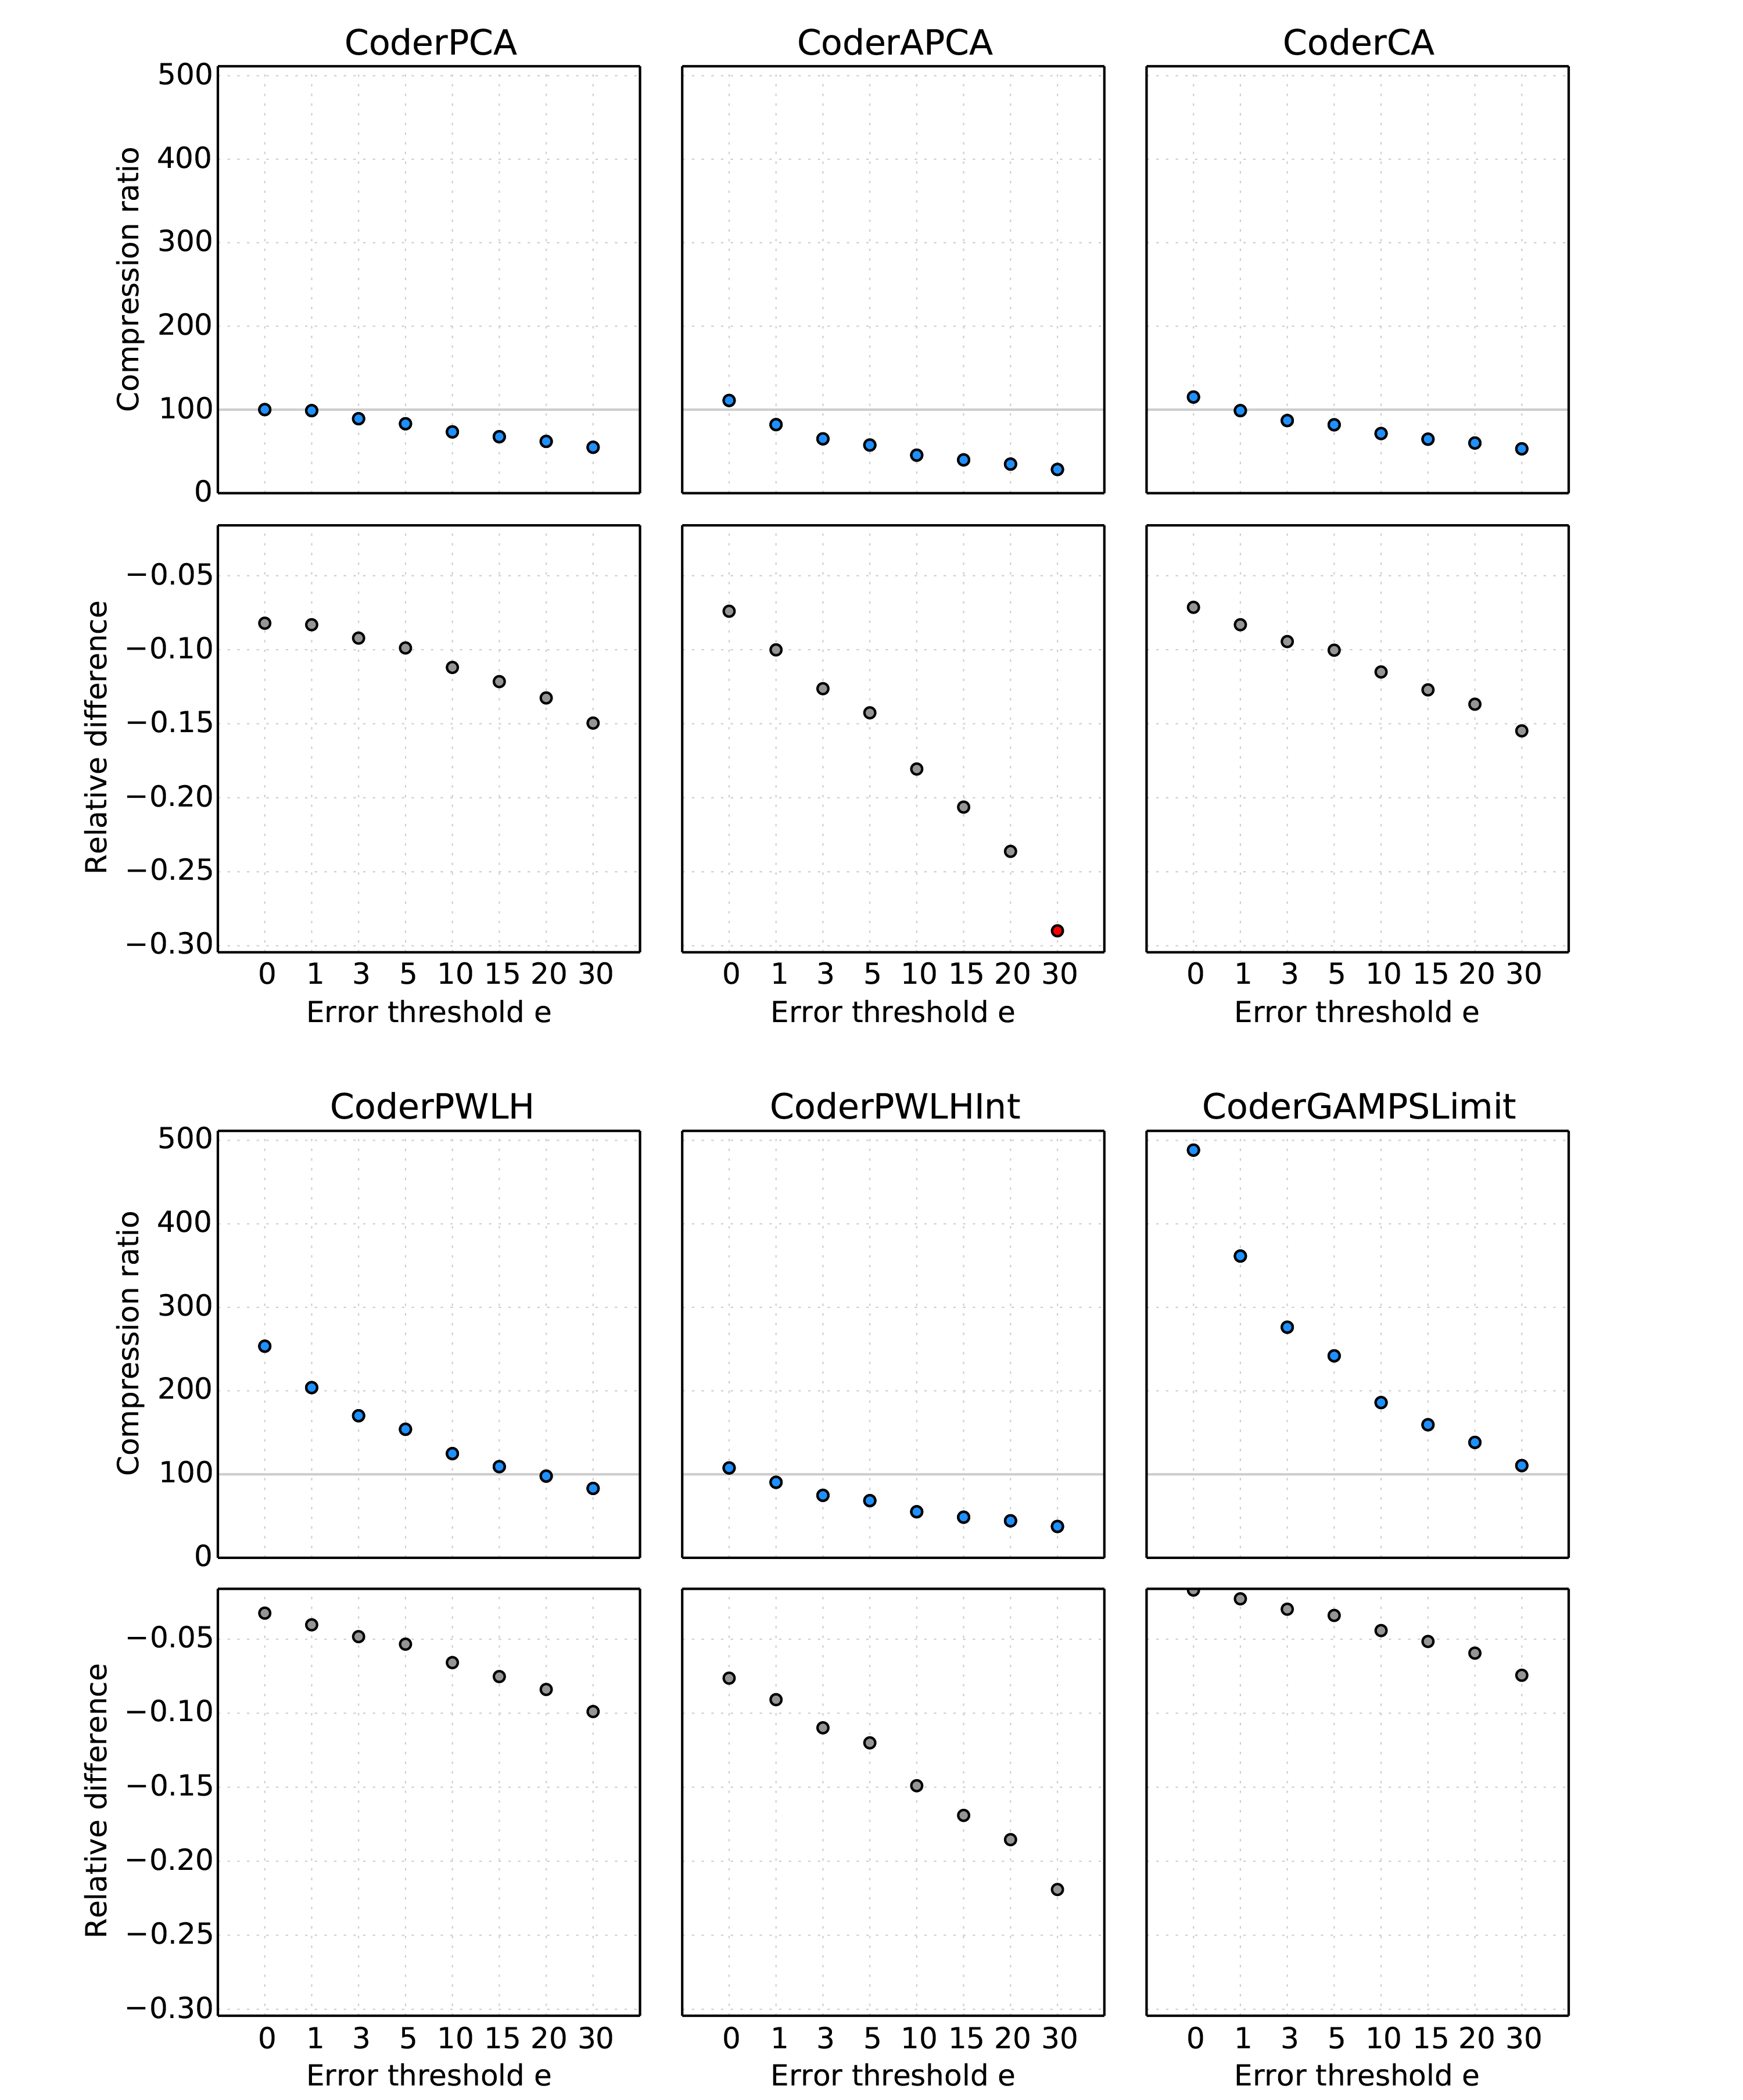
\includegraphics[scale=0.75]{chapters/Experiments/images/32-Tornado.png}
\hspace{+10pt}
\caption{\commonfigurescomp ``Longitude" data type of the \datasettornado \ dataset. In the relative difference plot for\\CoderAPCA we marked with red color the case in which \cNOmaskalgo \ obtains \\the most significant relative difference (-0.29).}
\label{fig:diff-tornado}
\end{figure}

\clearpage

\begin{figure}
\hspace{-70pt}
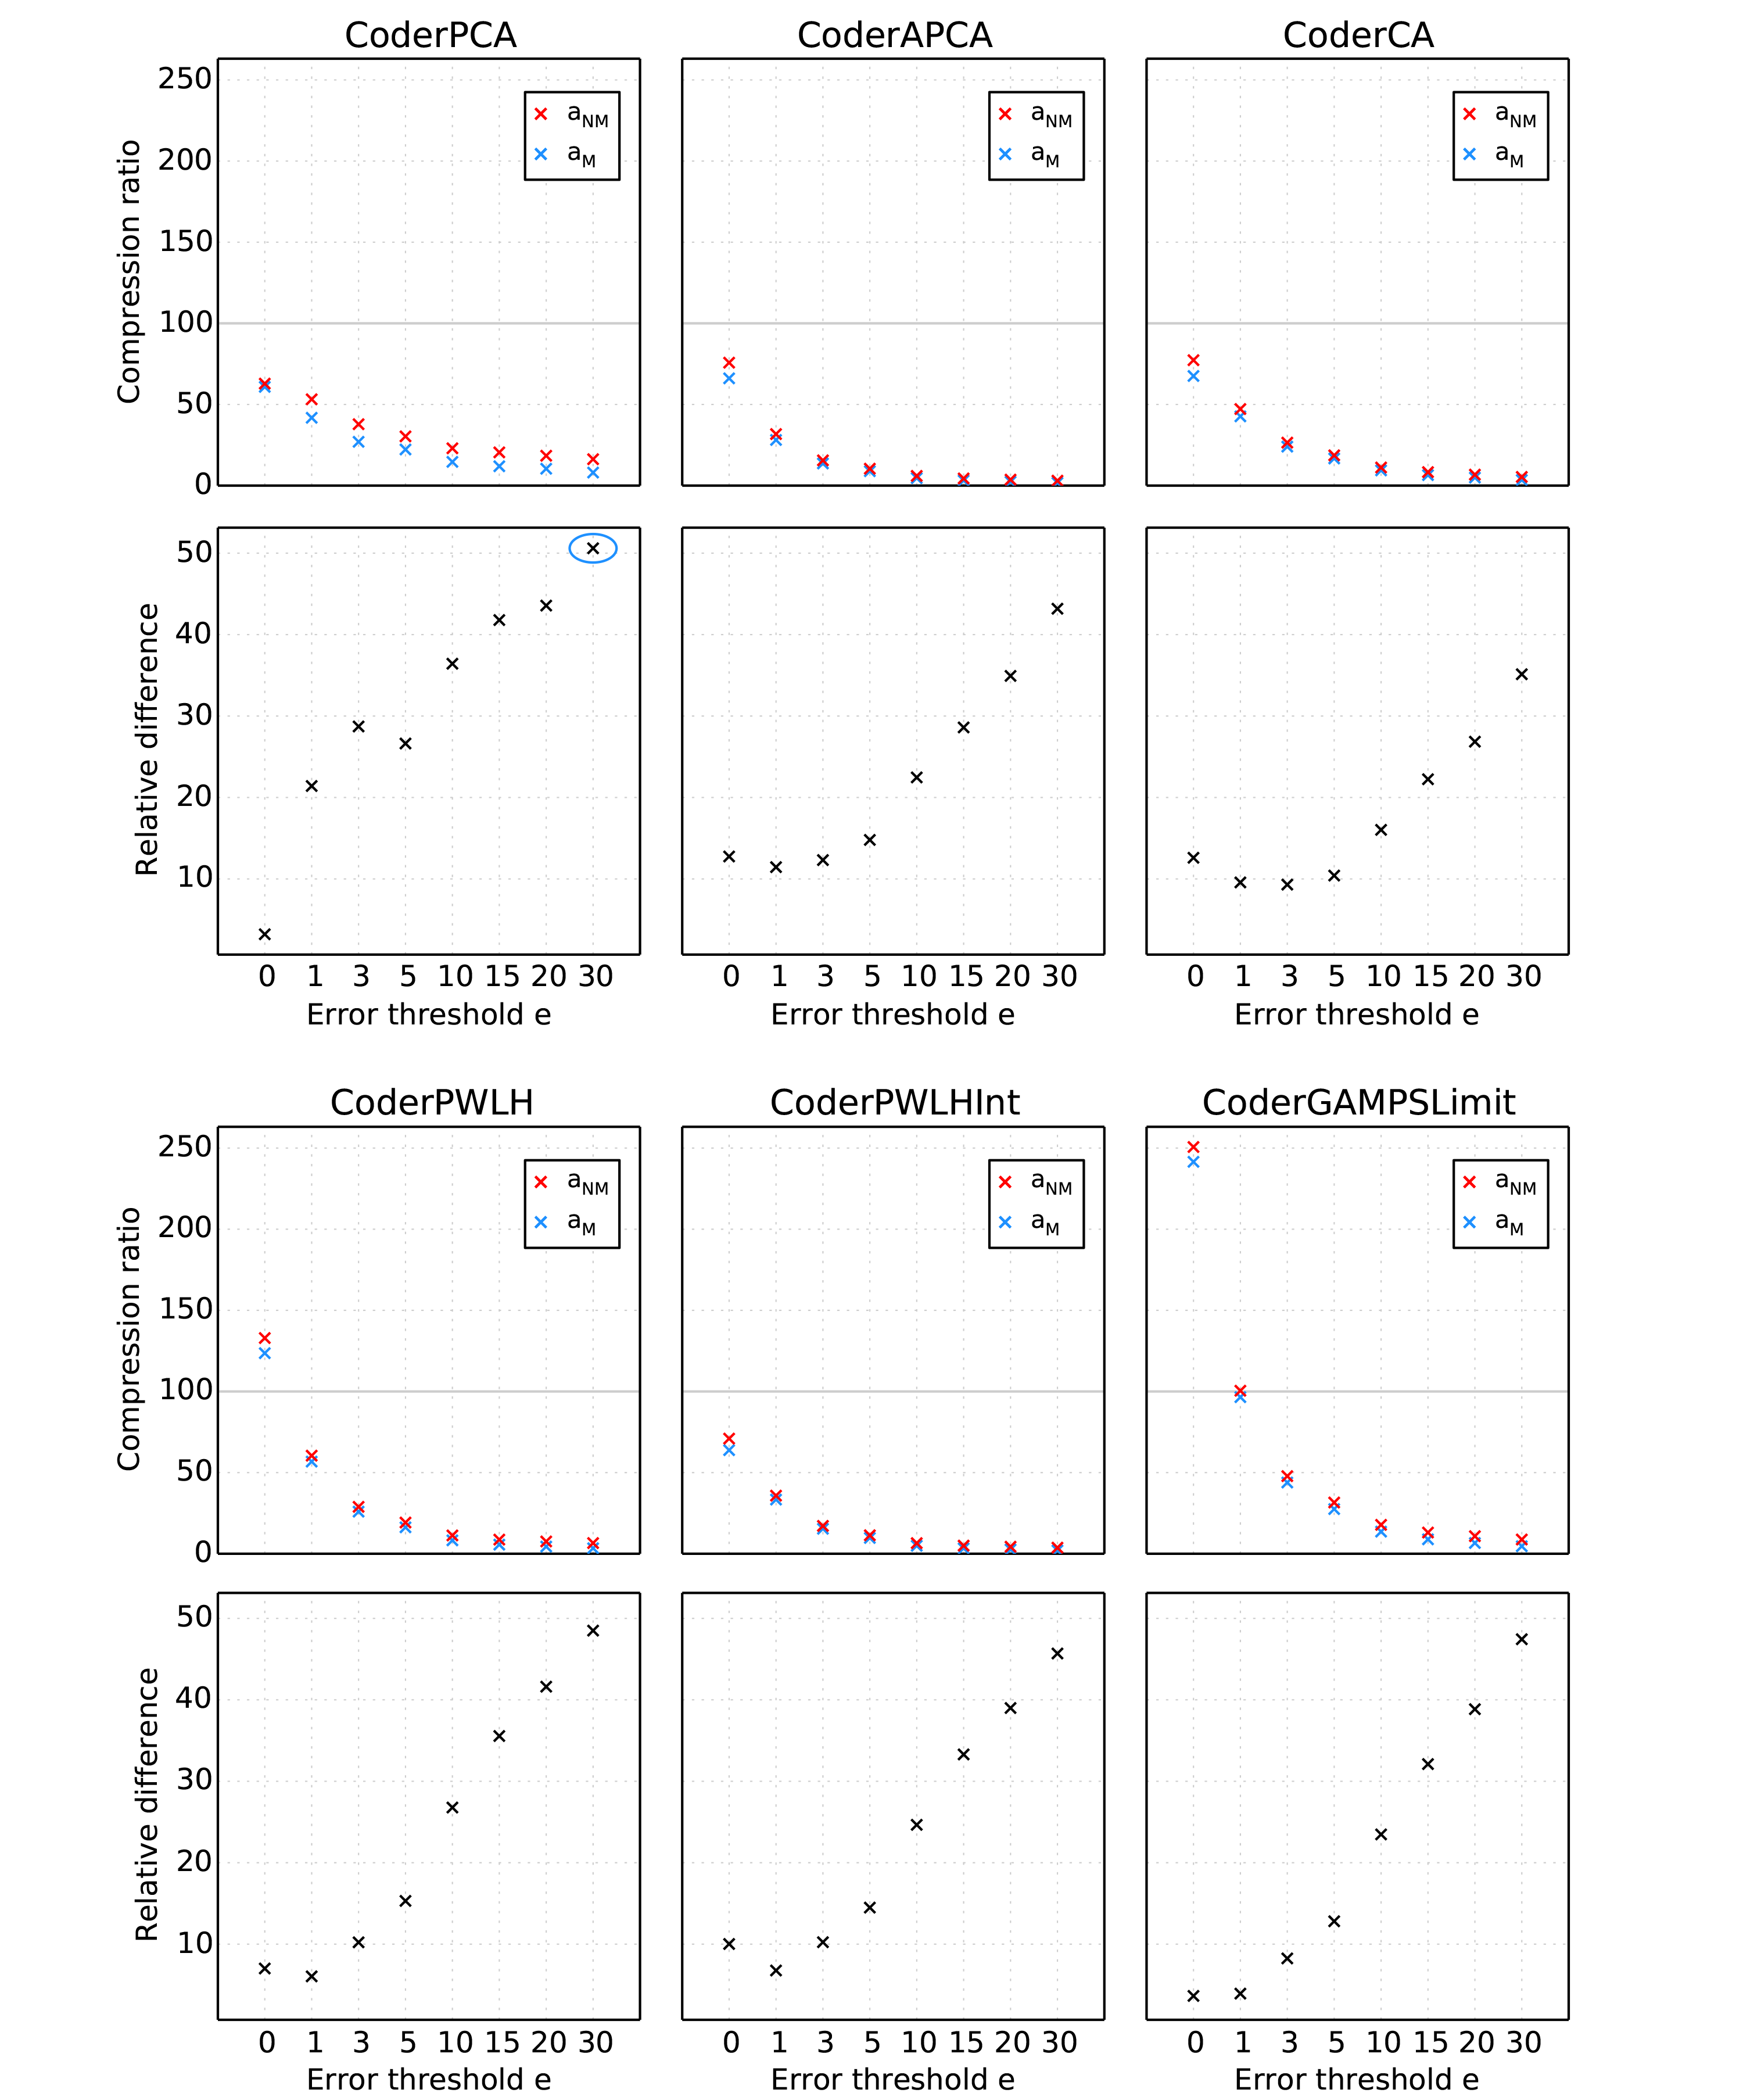
\includegraphics[scale=0.75]{chapters/Experiments/images/32-SST.png}
\hspace{+10pt}
\caption{\commonfigurescomp ``VWC" data type of the \datasetsst \ dataset. In the relative difference plot for\\CoderPCA we marked with blue color the case in which \cmaskalgo \ obtains \\the most significant relative difference (50.60).}
\label{fig:diff-sst}
\end{figure}


